\documentclass[10pt]{beamer}
\usetheme{metropolis}

% ── Packages ──
\usepackage{amsmath,amssymb,amsthm}
\usepackage{tikz}
\usetikzlibrary{positioning,arrows.meta}
\usepackage{graphicx}
\usepackage{array}

% ── Theorem environments ──
\theoremstyle{definition}
\newtheorem{defi}{Definition}[section]
\newtheorem{prop}{Proposition}[section]
\newtheorem{cor}{Corollary}[section]

\setbeamercolor{block title}{bg=red!75!black,fg=white}
\setbeamercolor{block body}{bg=yellow!10!white}

% ── Emoji definitions (used in introduction only) ──
\newcommand{\bean}{
\includegraphics[scale=0.07]{Pictures/bean.png}}
\newcommand{\leaf}{
\includegraphics[scale=0.08]{Pictures/leaf.png}}
\newcommand{\lemon}{
\includegraphics[scale=0.08]{Pictures/lemon.png}}
\newcommand{\cow}{
\includegraphics[scale=0.08]{Pictures/cow.png}}
\newcommand{\milk}{
\includegraphics[scale=0.07]{Pictures/milk.png}}
\newcommand{\coffee}{
\includegraphics[scale=0.10]{Pictures/coffee.png}}
\newcommand{\tea}{
\includegraphics[scale=0.08]{Pictures/tea.png}}
\newcommand{\bento}{
\includegraphics[scale=0.09]{Pictures/bento.png}}
\newcommand{\ramen}{
\includegraphics[scale=0.09]{Pictures/soup.png}}

% ── Cross-filling color commands (short names for AI maintainability) ──
\newcommand{\pvt}[1]{{\color{red}\mathbf{#1}}}       % pivot
\newcommand{\crs}[1]{{\color{blue}#1}}                % cross arm
\newcommand{\rem}[1]{{\color{gray}#1}}                % remainder zero

% ── Highlighting ──
\newcommand{\x}[1]{\alert{\textbf{#1}}}

\title{Cross-Filling Method}
\subtitle{Rank-One Decomposition and Sum $\leftrightarrow$ Product Equivalence}
\date{}

\begin{document}

\maketitle

% ═══════════════════════════════════════
% §0 INTRODUCTION
% ═══════════════════════════════════════
\section{Introduction}

\begin{frame}{Learning Objectives}
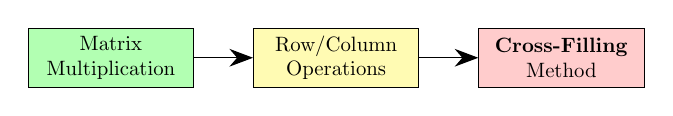
\begin{tikzpicture}[scale=0.75,transform shape,
    block/.style={draw, rectangle, minimum width=2.8cm, minimum height=1cm, align=center}]
\node[block,fill=green!30] (block1) {Matrix\\Multiplication};
\node[block, right=1cm of block1, fill=yellow!30] (block2) {Row/Column\\Operations};
\node[block, right=1cm of block2, fill=red!20] (block3) {\textbf{Cross-Filling}\\Method};
\draw[-{Stealth[length=3mm]}] (block1) -- (block2);
\draw[-{Stealth[length=3mm]}] (block2) -- (block3);
\end{tikzpicture}

\vspace{0.5cm}
\textbf{Key Questions:}
\begin{itemize}
\item What is a \x{rank-one matrix}?
\item How does \x{cross-filling} decompose any matrix into rank-one pieces?
\item How to convert between \x{sum form} and \x{product form}?
\item What is the \x{rank} of a matrix?
\end{itemize}
\end{frame}

\begin{frame}{Review: Sum-of-Rank-One View}
Recall from Lecture 1, matrix multiplication has a \x{sum-of-rank-one} view:
$$C =
\begin{pmatrix}
| & | & & | \\
a_1 & a_2 & \cdots & a_n \\
| & | & & |
\end{pmatrix}
\begin{pmatrix}
- & b_1^T & - \\
- & b_2^T & - \\
\vdots & \vdots & \vdots \\
- & b_n^T & -
\end{pmatrix}
= \sum_{k=1}^{n} a_k \, b_k^T$$

\vfill
Each $a_k \, b_k^T$ is a \x{rank-one matrix} (column $\times$ row).

\vfill
\textbf{Today's question}: Can we \x{reverse} this?

Given any matrix $C$, decompose it into rank-one pieces?
\end{frame}

\begin{frame}{Motivating Question}
\textbf{Coffee shop revisited:}

We have a direct recipe table:
$$C = \begin{array}{c|cc}
 & \text{\bento} & \text{\ramen} \\
\hline
\text{\leaf} & 2 & 2 \\
\text{\lemon} & 1 & 1 \\
\text{\bean} & 0 & 4 \\
\text{\cow} & 2 & 1
\end{array}$$

\textbf{Question}: Can we discover \x{hidden intermediate products} from just this table?

\vfill
The algorithm for doing this is called \x{cross-filling} (十字填充法).
\end{frame}

% ═══════════════════════════════════════
% §1 RANK-ONE MATRICES
% ═══════════════════════════════════════
\section{Rank-One Matrices}

\begin{frame}{Rank-One Matrix}
\begin{defi}
A matrix $R$ is \x{rank-one} if $R = \mathbf{u}\, \mathbf{v}^T$ for some nonzero column vector $\mathbf{u}$ and nonzero row vector $\mathbf{v}^T$.
\end{defi}

\vfill
Example:
$$R = \begin{pmatrix} 2 \\ 1 \\ 3 \end{pmatrix} \begin{pmatrix} 1 & 2 \end{pmatrix}
= \begin{pmatrix}
2 & 4 \\
1 & 2 \\
3 & 6
\end{pmatrix}$$

\vfill
All columns are multiples of $\mathbf{u} = (2,1,3)^T$.

All rows are multiples of $\mathbf{v}^T = (1,2)$.
\end{frame}

\begin{frame}{Recognizing Rank-One Structure}
Is this matrix rank-one?
$$\begin{pmatrix}
6 & 9 & 3 \\
4 & 6 & 2 \\
10 & 15 & 5
\end{pmatrix}$$

\vfill
Check rows:
\begin{itemize}
\item Row 1: $(6, 9, 3) = 3 \cdot (2, 3, 1)$
\item Row 2: $(4, 6, 2) = 2 \cdot (2, 3, 1)$
\item Row 3: $(10, 15, 5) = 5 \cdot (2, 3, 1)$
\end{itemize}

\vfill
Yes!\ \ $R = \begin{pmatrix} 3 \\ 2 \\ 5 \end{pmatrix} \begin{pmatrix} 2 & 3 & 1 \end{pmatrix}$.
\end{frame}

\begin{frame}{Cross-Product Equality}
In a rank-one matrix $R = \mathbf{u}\,\mathbf{v}^T$, every entry is $r_{ij} = u_i v_j$.

\vfill
For any four entries forming a rectangle:
$$\boxed{r_{ij} \cdot r_{k\ell} = r_{i\ell} \cdot r_{kj}}$$

\vfill
\textbf{Why?}\ \ $(u_i v_j)(u_k v_\ell) = (u_i v_\ell)(u_k v_j) = u_i u_k v_j v_\ell$.

\vfill
\textbf{Check}: In $\begin{pmatrix} 6 & 9 \\ 4 & 6 \end{pmatrix}$: \quad $6 \times 6 = 36 = 9 \times 4$ \quad $\checkmark$
\end{frame}

\begin{frame}{Not Every Matrix is Rank-One}
$$C = \begin{pmatrix}
2 & 4 \\
1 & 2 \\
3 & 7
\end{pmatrix}$$

\vfill
Check ratios: $\frac{4}{2} = 2$, \quad $\frac{2}{1} = 2$, \quad $\frac{7}{3} \neq 2$ \quad $\leftarrow$ Different!

\vfill
This is \x{not rank-one}. But can we write it as a \x{sum} of rank-one pieces?

$$C = \underbrace{\begin{pmatrix} ? \end{pmatrix}}_{R_1} + \underbrace{\begin{pmatrix} ? \end{pmatrix}}_{R_2}$$
\end{frame}

% ═══════════════════════════════════════
% §2 ONE-STEP CROSS-FILLING
% ═══════════════════════════════════════
\section{Cross-Filling: One Step}

\begin{frame}{Step 1: Choose a Pivot}
$$C = \begin{pmatrix}
2 & 4 \\
1 & 2 \\
3 & 7
\end{pmatrix}$$

\vfill
Choose any nonzero entry as the \x{pivot}. We pick $c_{11} = 2$:

$$C = \begin{pmatrix}
\pvt{2} & 4 \\
1 & 2 \\
3 & 7
\end{pmatrix}$$
\end{frame}

\begin{frame}{Step 2: Extract the Cross}
The \x{cross} through the pivot: its entire \x{row} and \x{column}.

$$C = \begin{pmatrix}
\pvt{2} & \crs{4} \\
\crs{1} & 2 \\
\crs{3} & 7
\end{pmatrix}$$

\vfill
\begin{itemize}
\item Cross row: $\begin{pmatrix} \pvt{2} & \crs{4} \end{pmatrix}$
\item Cross column: $\begin{pmatrix} \pvt{2} \\ \crs{1} \\ \crs{3} \end{pmatrix}$
\end{itemize}
\end{frame}

\begin{frame}{Step 3: Fill Using the Cross}
Build a rank-one matrix using the \x{multiplication table} principle:
$$R_{k\ell} = \frac{(\text{column})_k \times (\text{row})_\ell}{\text{pivot}}$$

\vfill
\begin{align*}
R_{11} &= \frac{\crs{2} \times \crs{2}}{\pvt{2}} = 2 &
R_{12} &= \frac{\crs{2} \times \crs{4}}{\pvt{2}} = 4 \\[4pt]
R_{21} &= \frac{\crs{1} \times \crs{2}}{\pvt{2}} = 1 &
R_{22} &= \frac{\crs{1} \times \crs{4}}{\pvt{2}} = 2 \\[4pt]
R_{31} &= \frac{\crs{3} \times \crs{2}}{\pvt{2}} = 3 &
R_{32} &= \frac{\crs{3} \times \crs{4}}{\pvt{2}} = 6
\end{align*}
\end{frame}

\begin{frame}{The Rank-One Piece $R_1$}
$$R_1 = \begin{pmatrix}
\pvt{2} & \crs{4} \\
\crs{1} & 2 \\
\crs{3} & 6
\end{pmatrix}
= \frac{1}{\pvt{2}}
\begin{pmatrix} \crs{2} \\ \crs{1} \\ \crs{3} \end{pmatrix}
\begin{pmatrix} \crs{2} & \crs{4} \end{pmatrix}$$

\vfill
This is $\mathbf{u}_1 \mathbf{v}_1^T$ — a rank-one matrix built entirely from the cross!
\end{frame}

\begin{frame}{Step 4: Compute the Remainder}
$$C - R_1 = \begin{pmatrix}
2 & 4 \\
1 & 2 \\
3 & 7
\end{pmatrix}
- \begin{pmatrix}
2 & 4 \\
1 & 2 \\
3 & 6
\end{pmatrix}
= \begin{pmatrix}
\rem{0} & \rem{0} \\
\rem{0} & \rem{0} \\
\rem{0} & 1
\end{pmatrix}$$

\vfill
Key: The \x{entire cross region} (row~1 and column~1) is now \x{zero}!

\vfill
This is why it is called ``cross-filling'' — the cross is \x{filled in} and eliminated.
\end{frame}

\begin{frame}{Step 5: The Remainder is Simpler}
The remainder $C_2 = \begin{pmatrix}
\rem{0} & \rem{0} \\
\rem{0} & \rem{0} \\
\rem{0} & 1
\end{pmatrix}$ is already rank-one:

$$R_2 = \begin{pmatrix} 0 \\ 0 \\ 1 \end{pmatrix}\begin{pmatrix} 0 & 1 \end{pmatrix}$$

\vfill
\textbf{Final decomposition:}
$$\underbrace{\begin{pmatrix}
2 & 4 \\
1 & 2 \\
3 & 7
\end{pmatrix}}_{C}
= \underbrace{\begin{pmatrix}
\pvt{2} & \crs{4} \\
\crs{1} & 2 \\
\crs{3} & 6
\end{pmatrix}}_{R_1}
+ \underbrace{\begin{pmatrix}
\rem{0} & \rem{0} \\
\rem{0} & \rem{0} \\
\rem{0} & \pvt{1}
\end{pmatrix}}_{R_2}$$
\end{frame}

\begin{frame}{Why ``Cross-Filling''?}
\begin{center}
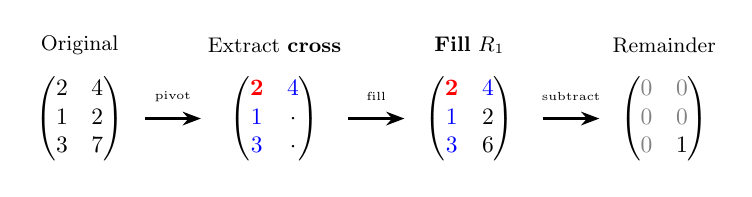
\begin{tikzpicture}[scale=0.55, every node/.style={scale=0.85}]
% Step 1: Original
\node at (0,3.2) {\small Original};
\node at (0,1.5) {$\begin{pmatrix} 2 & 4 \\ 1 & 2 \\ 3 & 7 \end{pmatrix}$};

% Arrow
\draw[-{Stealth},thick] (1.5,1.5) -- (2.8,1.5);
\node at (2.15,2) {\tiny pivot};

% Step 2: Cross
\node at (4.5,3.2) {\small Extract \x{cross}};
\node at (4.5,1.5) {$\begin{pmatrix} \pvt{2} & \crs{4} \\ \crs{1} & \cdot \\ \crs{3} & \cdot \end{pmatrix}$};

% Arrow
\draw[-{Stealth},thick] (6.2,1.5) -- (7.5,1.5);
\node at (6.85,2) {\tiny fill};

% Step 3: Filled
\node at (9,3.2) {\small \x{Fill} $R_1$};
\node at (9,1.5) {$\begin{pmatrix} \pvt{2} & \crs{4} \\ \crs{1} & 2 \\ \crs{3} & 6 \end{pmatrix}$};

% Arrow
\draw[-{Stealth},thick] (10.7,1.5) -- (12,1.5);
\node at (11.35,2) {\tiny subtract};

% Step 4: Remainder
\node at (13.5,3.2) {\small Remainder};
\node at (13.5,1.5) {$\begin{pmatrix} \rem{0} & \rem{0} \\ \rem{0} & \rem{0} \\ \rem{0} & 1 \end{pmatrix}$};
\end{tikzpicture}
\end{center}

\vfill
\begin{enumerate}
\item Choose \pvt{pivot} (center of cross)
\item Extract \crs{cross} (row $+$ column through pivot)
\item \x{Fill} all entries via multiplication table
\item Subtract $\to$ cross region becomes \rem{zero}
\end{enumerate}
\end{frame}

\begin{frame}{One-Step Cross-Filling: Formula}
\begin{prop}
Let $A$ be a matrix with $a_{ij} \neq 0$. The rank-one piece from cross-filling at pivot position $(i,j)$:
$$R = \frac{1}{a_{ij}} \cdot (\text{column } j \text{ of } A) \cdot (\text{row } i \text{ of } A)$$
\end{prop}

\vfill
After subtracting $R$ from $A$:
\begin{itemize}
\item Row $i$ of $A - R$ is all zeros
\item Column $j$ of $A - R$ is all zeros
\end{itemize}

\vfill
The cross through $(i,j)$ is \x{eliminated}.
\end{frame}

% ═══════════════════════════════════════
% §3 FULL ALGORITHM: 3×3 EXAMPLE
% ═══════════════════════════════════════
\section{Cross-Filling Algorithm}

\begin{frame}{A $3 \times 3$ Example}
Decompose the following matrix by cross-filling:
$$A = \begin{pmatrix}
1 & 1 & 1 \\
1 & 3 & 3 \\
1 & 3 & 8
\end{pmatrix}$$

\vfill
We will peel off rank-one pieces iteratively until nothing remains.
\end{frame}

\begin{frame}{Iteration 1: Pivot $a_{11} = 1$}
Highlight the cross through $a_{11}$:
$$A = \begin{pmatrix}
\pvt{1} & \crs{1} & \crs{1} \\
\crs{1} & 3 & 3 \\
\crs{1} & 3 & 8
\end{pmatrix}$$

\vfill
Fill using the cross:
$$R_1 = \frac{1}{\pvt{1}}
\begin{pmatrix} \crs{1} \\ \crs{1} \\ \crs{1} \end{pmatrix}
\begin{pmatrix} \crs{1} & \crs{1} & \crs{1} \end{pmatrix}
= \begin{pmatrix}
\pvt{1} & \crs{1} & \crs{1} \\
\crs{1} & 1 & 1 \\
\crs{1} & 1 & 1
\end{pmatrix}$$
\end{frame}

\begin{frame}{Iteration 1: Remainder $A_1$}
$$A_1 = A - R_1 = \begin{pmatrix}
1 & 1 & 1 \\
1 & 3 & 3 \\
1 & 3 & 8
\end{pmatrix}
- \begin{pmatrix}
1 & 1 & 1 \\
1 & 1 & 1 \\
1 & 1 & 1
\end{pmatrix}
= \begin{pmatrix}
\rem{0} & \rem{0} & \rem{0} \\
\rem{0} & 2 & 2 \\
\rem{0} & 2 & 7
\end{pmatrix}$$

\vfill
Row 1 and column 1 are now \rem{zero}.\ \ $\checkmark$
\end{frame}

\begin{frame}{Iteration 2: Pivot $(A_1)_{22} = 2$}
$$A_1 = \begin{pmatrix}
\rem{0} & \rem{0} & \rem{0} \\
\rem{0} & \pvt{2} & \crs{2} \\
\rem{0} & \crs{2} & 7
\end{pmatrix}$$

\vfill
Fill using the new cross:
$$R_2 = \frac{1}{\pvt{2}}
\begin{pmatrix} \rem{0} \\ \crs{2} \\ \crs{2} \end{pmatrix}
\begin{pmatrix} \rem{0} & \crs{2} & \crs{2} \end{pmatrix}
= \begin{pmatrix}
\rem{0} & \rem{0} & \rem{0} \\
\rem{0} & \pvt{2} & \crs{2} \\
\rem{0} & \crs{2} & 2
\end{pmatrix}$$
\end{frame}

\begin{frame}{Iteration 2: Remainder $A_2$}
$$A_2 = A_1 - R_2 = \begin{pmatrix}
0 & 0 & 0 \\
0 & 2 & 2 \\
0 & 2 & 7
\end{pmatrix}
- \begin{pmatrix}
0 & 0 & 0 \\
0 & 2 & 2 \\
0 & 2 & 2
\end{pmatrix}
= \begin{pmatrix}
\rem{0} & \rem{0} & \rem{0} \\
\rem{0} & \rem{0} & \rem{0} \\
\rem{0} & \rem{0} & 5
\end{pmatrix}$$

\vfill
Rows 1--2 and columns 1--2 are now \rem{zero}.\ \ $\checkmark$
\end{frame}

\begin{frame}{Iteration 3: Final Piece}
$$A_2 = \begin{pmatrix}
\rem{0} & \rem{0} & \rem{0} \\
\rem{0} & \rem{0} & \rem{0} \\
\rem{0} & \rem{0} & \pvt{5}
\end{pmatrix}$$

\vfill
This is already rank-one:
$$R_3 = \begin{pmatrix} 0 \\ 0 \\ 1 \end{pmatrix}
\begin{pmatrix} 0 & 0 & 5 \end{pmatrix}
= \begin{pmatrix}
\rem{0} & \rem{0} & \rem{0} \\
\rem{0} & \rem{0} & \rem{0} \\
\rem{0} & \rem{0} & \pvt{5}
\end{pmatrix}$$

Remainder: $A_3 = A_2 - R_3 = O$. \quad \x{Done!}
\end{frame}

\begin{frame}{Full Decomposition}
$$A = \underbrace{\begin{pmatrix}
\pvt{1} & \crs{1} & \crs{1} \\
\crs{1} & 1 & 1 \\
\crs{1} & 1 & 1
\end{pmatrix}}_{R_1}
+ \underbrace{\begin{pmatrix}
\rem{0} & \rem{0} & \rem{0} \\
\rem{0} & \pvt{2} & \crs{2} \\
\rem{0} & \crs{2} & 2
\end{pmatrix}}_{R_2}
+ \underbrace{\begin{pmatrix}
\rem{0} & \rem{0} & \rem{0} \\
\rem{0} & \rem{0} & \rem{0} \\
\rem{0} & \rem{0} & \pvt{5}
\end{pmatrix}}_{R_3}$$

\vfill
Three rank-one pieces:
\begin{itemize}
\item $R_1$: pivot $\pvt{1}$ at position $(1,1)$
\item $R_2$: pivot $\pvt{2}$ at position $(2,2)$
\item $R_3$: pivot $\pvt{5}$ at position $(3,3)$
\end{itemize}
\end{frame}

\begin{frame}{The Cross-Filling Algorithm}
\begin{prop}[Cross-Filling Algorithm]
\textbf{Input}: Matrix $A$ ($m \times n$).

\textbf{Output}: $A = R_1 + R_2 + \cdots + R_r$ (sum of rank-one matrices).

\textbf{Procedure}:
\begin{enumerate}
\item Find any nonzero entry $a_{ij} \neq 0$ (the \x{pivot}).
\item Form rank-one piece:
$$R = \frac{1}{a_{ij}} \cdot (\text{column } j) \cdot (\text{row } i)$$
\item Compute remainder $A' = A - R$.
\item Repeat on $A'$ until $A' = O$.
\end{enumerate}
\end{prop}

\vfill
Each step eliminates one cross (one row and one column become zero).
\end{frame}

\begin{frame}{Rank of a Matrix}
\begin{defi}
The \x{rank} of a matrix $A$ is the number of rank-one pieces in its cross-filling decomposition:
$$A = R_1 + R_2 + \cdots + R_r \quad \Longrightarrow \quad \operatorname{rank}(A) = r$$
\end{defi}

\vfill
\textbf{Examples:}
\begin{itemize}
\item Zero matrix $O$: rank $0$
\item Rank-one matrix $\mathbf{u}\mathbf{v}^T$: rank $1$
\item Identity $I_n$: rank $n$
\item Our $A$ above: rank $3$
\end{itemize}

\vfill
\textbf{Warning}: Different pivot choices give different decompositions. Do they always give the same count? \x{Yes} — but we prove this in Lecture 4.
\end{frame}

% ═══════════════════════════════════════
% §4 SUM ↔ PRODUCT EQUIVALENCE
% ═══════════════════════════════════════
\section{Sum $\leftrightarrow$ Product Equivalence}

\begin{frame}{Outer Product Recap}
Each rank-one piece is an \x{outer product} (column $\times$ row):
$$R_k = \mathbf{u}_k \, \mathbf{v}_k^T$$

\vfill
\begin{center}
\begin{tabular}{c|c|c}
 & Inner product & Outer product \\
\hline
Form & $\mathbf{u}^T \mathbf{v}$ (row $\times$ col) & $\mathbf{u}\,\mathbf{v}^T$ (col $\times$ row) \\
Result & scalar & matrix \\
Size & $(1\!\times\! n)(n\!\times\! 1) = 1\!\times\! 1$ & $(m\!\times\! 1)(1\!\times\! n) = m\!\times\! n$
\end{tabular}
\end{center}

\vfill
Cross-filling produces \x{outer products} — each is a rank-one matrix.
\end{frame}

\begin{frame}{Collecting the Pieces}
From our $3\times 3$ example:
\begin{align*}
R_1 &= \underbrace{\begin{pmatrix} 1 \\ 1 \\ 1 \end{pmatrix}}_{\mathbf{u}_1}
\underbrace{\begin{pmatrix} 1 & 1 & 1 \end{pmatrix}}_{\mathbf{v}_1^T} \\[6pt]
R_2 &= \underbrace{\begin{pmatrix} 0 \\ 1 \\ 1 \end{pmatrix}}_{\mathbf{u}_2}
\underbrace{\begin{pmatrix} 0 & 2 & 2 \end{pmatrix}}_{\mathbf{v}_2^T} \\[6pt]
R_3 &= \underbrace{\begin{pmatrix} 0 \\ 0 \\ 1 \end{pmatrix}}_{\mathbf{u}_3}
\underbrace{\begin{pmatrix} 0 & 0 & 5 \end{pmatrix}}_{\mathbf{v}_3^T}
\end{align*}
\end{frame}

\begin{frame}{Product Form: $A = UV$}
Collect columns $\mathbf{u}_k$ into $U$, rows $\mathbf{v}_k^T$ into $V$:
$$U = \begin{pmatrix}
| & | & | \\
\mathbf{u}_1 & \mathbf{u}_2 & \mathbf{u}_3 \\
| & | & |
\end{pmatrix}
= \begin{pmatrix}
1 & 0 & 0 \\
1 & 1 & 0 \\
1 & 1 & 1
\end{pmatrix}$$
$$V = \begin{pmatrix}
- & \mathbf{v}_1^T & - \\
- & \mathbf{v}_2^T & - \\
- & \mathbf{v}_3^T & -
\end{pmatrix}
= \begin{pmatrix}
1 & 1 & 1 \\
0 & 2 & 2 \\
0 & 0 & 5
\end{pmatrix}$$

By sum-of-rank-one:\ \ $UV = \sum_{k=1}^{3} \mathbf{u}_k\, \mathbf{v}_k^T = R_1 + R_2 + R_3 = A$.
\end{frame}

\begin{frame}{Verification}
$$UV = \begin{pmatrix}
1 & 0 & 0 \\
1 & 1 & 0 \\
1 & 1 & 1
\end{pmatrix}
\begin{pmatrix}
1 & 1 & 1 \\
0 & 2 & 2 \\
0 & 0 & 5
\end{pmatrix}
= \begin{pmatrix}
1 & 1 & 1 \\
1 & 3 & 3 \\
1 & 3 & 8
\end{pmatrix} = A \quad \checkmark$$

\vfill
Notice: $U$ is \x{lower triangular}, $V$ is \x{upper triangular}!

\vfill
This happened because we chose \x{diagonal pivots} $(1,1) \to (2,2) \to (3,3)$.

\vfill
Diagonal pivots $\Longrightarrow$ the product form is an \x{LU decomposition}.
\end{frame}

\begin{frame}{Sum $\leftrightarrow$ Product Equivalence}
\begin{prop}
For any matrix $A$:
$$A = \sum_{k=1}^r \mathbf{u}_k\,\mathbf{v}_k^T \quad \Longleftrightarrow \quad A = U \cdot V$$
where $U$ has columns $\mathbf{u}_k$ and $V$ has rows $\mathbf{v}_k^T$.
\end{prop}

\vfill
Two directions:
\begin{itemize}
\item \textbf{Lecture 1}: Given product $A = UV$, read off sum $A = \sum \mathbf{u}_k\,\mathbf{v}_k^T$
\item \textbf{Today}: Given sum from cross-filling, assemble product $A = UV$
\end{itemize}
\end{frame}

\begin{frame}{The Inner Dimension}
When $A = UV$ with $A$ being $m \times n$:
$$A_{m \times n} = U_{m \times \boxed{r}} \cdot V_{\boxed{r} \times n}$$

The shared dimension $r$ is the \x{inner dimension}.

\vfill
\begin{itemize}
\item Outer dimensions $m, n$: visible (size of $A$)
\item Inner dimension $r$: \x{hidden} = number of independent patterns
\end{itemize}

\vfill
Key: $\operatorname{rank}(A) = r$ = inner dimension of the factorization.
\end{frame}

% ═══════════════════════════════════════
% §5 ALGEBRAIC EXPRESSION
% ═══════════════════════════════════════
\section{Algebraic Expression for Cross-Filling}

\begin{frame}{Cross-Filling as a Matrix Formula}
Let $e_i$ be the $i$-th column of $I_n$, and $e_j^T$ the $j$-th row of $I_m$.

\vfill
Then:
\begin{itemize}
\item $Ae_i$ = column $i$ of $A$
\item $e_j^T A$ = row $j$ of $A$
\item $e_j^T A e_i$ = entry $(j,i)$ of $A$ = the pivot
\end{itemize}

\vfill
The cross-filling formula at pivot position (row $j$, column $i$):
$$\boxed{R = A e_i \, (e_j^T A e_i)^{-1} \, e_j^T A}$$

\vfill
This is: $\dfrac{1}{\text{pivot}} \times \text{(column)} \times \text{(row)}$.
\end{frame}

\begin{frame}{Example Verification}
$A = \begin{pmatrix} 1 & 1 & 1 \\ 1 & 3 & 3 \\ 1 & 3 & 8 \end{pmatrix}$, \quad cross-fill at row 1, column 1:

\vfill
\begin{align*}
Ae_1 &= \begin{pmatrix} 1 \\ 1 \\ 1 \end{pmatrix}, \quad
e_1^T A = \begin{pmatrix} 1 & 1 & 1 \end{pmatrix}, \quad
e_1^T A e_1 = 1
\end{align*}

$$R_1 = \begin{pmatrix} 1 \\ 1 \\ 1 \end{pmatrix} \cdot 1 \cdot \begin{pmatrix} 1 & 1 & 1 \end{pmatrix}
= \begin{pmatrix}
1 & 1 & 1 \\
1 & 1 & 1 \\
1 & 1 & 1
\end{pmatrix} \quad \checkmark$$
\end{frame}

\begin{frame}{Application: Projection Matrices}
\begin{defi}
A square matrix $P$ is a \x{projection} if $P^2 = P$.
\end{defi}

\vfill
\begin{prop}
If $P$ is a projection and $R$ is obtained by cross-filling from $P$, then $R$ is also a projection.
\end{prop}

\vfill
\textbf{Proof}: Let $R = Pe_i(e_j^TPe_i)^{-1}e_j^TP$. Then
\begin{align*}
R^2 &= Pe_i(e_j^TPe_i)^{-1} \underbrace{e_j^T P \cdot P e_i}_{= \, e_j^TPe_i} (e_j^TPe_i)^{-1}e_j^TP \\
&= Pe_i(e_j^TPe_i)^{-1}e_j^TP = R \quad \checkmark
\end{align*}

(Used $P^2 = P$ in the underbraced step.)
\end{frame}

\begin{frame}{Projection Decomposition}
If $P$ is a projection and $R$ comes from cross-filling $P$:
$$P = \underbrace{R}_{\text{projection}} + \underbrace{(P-R)}_{\text{also projection!}}$$

\vfill
Check: $(P-R)^2 = P^2 + R^2 - PR - RP = P + R - R - R = P - R$ \quad $\checkmark$

\vfill
(Here $PR = QP = R$ since $P^2 = P$ implies columns and rows of $P$ are fixed by $P$.)

\vfill
Cross-filling \x{decomposes projections into smaller projections}.

This will be \x{extremely important} for spectral decomposition.
\end{frame}

% ═══════════════════════════════════════
% §6 PREVIEW: LU DECOMPOSITION
% ═══════════════════════════════════════
\section{Preview: LU Decomposition}

\begin{frame}{Diagonal Pivots $\Rightarrow$ LU}
In our example, diagonal pivots produced:
$$A = \underbrace{\begin{pmatrix}
1 & 0 & 0 \\
1 & 1 & 0 \\
1 & 1 & 1
\end{pmatrix}}_{\text{lower triangular } L}
\underbrace{\begin{pmatrix}
1 & 1 & 1 \\
0 & 2 & 2 \\
0 & 0 & 5
\end{pmatrix}}_{\text{upper triangular } U}$$

\vfill
Key: The pivots $\pvt{1}, \pvt{2}, \pvt{5}$ appear on the diagonal of $U$.

\vfill
Diagonal cross-filling $\Longrightarrow$ \x{LU decomposition}.
\end{frame}

\begin{frame}{LDU Decomposition}
We can further separate the pivots into a diagonal matrix:
$$A = \underbrace{\begin{pmatrix}
1 & 0 & 0 \\
1 & 1 & 0 \\
1 & 1 & 1
\end{pmatrix}}_{L}
\underbrace{\begin{pmatrix}
\pvt{1} & 0 & 0 \\
0 & \pvt{2} & 0 \\
0 & 0 & \pvt{5}
\end{pmatrix}}_{D}
\underbrace{\begin{pmatrix}
1 & 1 & 1 \\
0 & 1 & 1 \\
0 & 0 & 1
\end{pmatrix}}_{U}$$

\vfill
\begin{itemize}
\item $L$: lower triangular, 1's on diagonal (from normalized cross columns)
\item $D$: diagonal matrix of \x{pivots} (the cross centers)
\item $U$: upper triangular, 1's on diagonal (from normalized cross rows)
\end{itemize}

\vfill
Each rank-one piece: $R_k = L D_k U$ where $D_k$ keeps only the $k$-th pivot.
\end{frame}

\begin{frame}{Not All Matrices Are LDU-Decomposable}
Diagonal cross-filling requires \x{nonzero diagonal pivots}. But this can fail:

$$A = \begin{pmatrix} 0 & 3 \\ 1 & 2 \end{pmatrix}$$

Pivot $a_{11} = 0$ — cannot start!

\vfill
Even later pivots can fail:
$$\begin{pmatrix} 1 & 2 & 3 \\ 1 & 2 & 4 \\ 1 & 3 & 5 \end{pmatrix}
\xrightarrow{\text{after } R_1} \begin{pmatrix}
\rem{0} & \rem{0} & \rem{0} \\
\rem{0} & \pvt{0} & 1 \\
\rem{0} & 1 & 2
\end{pmatrix}$$

Second pivot is \pvt{zero}!

\vfill
\textbf{Solution}: Allow non-diagonal pivots, or permute rows first $\to$ \x{PLU decomposition} (future lecture).
\end{frame}

% ═══════════════════════════════════════
% §7 EXERCISES
% ═══════════════════════════════════════
\section{Exercises}

\begin{frame}{Exercise 1}
\textbf{Exercise 1.1}: Cross-fill the following matrix. How many rank-one pieces are needed?
$$A = \begin{pmatrix}
2 & 6 & 4 \\
1 & 3 & 2
\end{pmatrix}$$

\vfill

\textbf{Exercise 1.2}: Cross-fill using diagonal pivots, and write the result as $A = LU$.
$$B = \begin{pmatrix}
2 & 4 & 2 \\
1 & 3 & 2 \\
4 & 10 & 8
\end{pmatrix}$$
\end{frame}

\begin{frame}{Exercise 2}
\textbf{Exercise 1.3}: Let $A$ be an $m \times n$ matrix with $\operatorname{rank}(A) = r$.

\vfill

(a) Explain why $r \leq \min(m, n)$.

\vfill

(b) Show that $A = UV$ where $U$ is $m \times r$ and $V$ is $r \times n$.
\end{frame}

\begin{frame}{Exercise 3}
\textbf{Exercise 1.4}: Let $P$ be a $3\times 3$ projection matrix ($P^2 = P$):
$$P = \begin{pmatrix}
\frac{1}{2} & \frac{1}{2} & 0 \\[3pt]
\frac{1}{2} & \frac{1}{2} & 0 \\[3pt]
0 & 0 & 1
\end{pmatrix}$$

\vfill

(a) Cross-fill at pivot $p_{11} = \frac{1}{2}$. Find the rank-one piece $R$.

\vfill

(b) Verify $R^2 = R$.

\vfill

(c) Verify $(P-R)^2 = P - R$.
\end{frame}

% ═══════════════════════════════════════
% SUMMARY
% ═══════════════════════════════════════

\begin{frame}{Summary}
\textbf{Today we learned:}

\begin{enumerate}
\item \textbf{Rank-one matrix}: $R = \mathbf{u}\,\mathbf{v}^T$ (one pattern, repeated)

\item \textbf{Cross-filling algorithm}: Decompose any matrix into rank-one pieces
$$A = R_1 + R_2 + \cdots + R_r$$

\item \textbf{Sum $\leftrightarrow$ Product}:
$$\sum_{k=1}^r \mathbf{u}_k\,\mathbf{v}_k^T = A = UV$$

\item \textbf{Rank} = number of pieces = inner dimension of $UV$

\item \textbf{Algebraic formula}: $R = Ae_i(e_j^TAe_i)^{-1}e_j^TA$

\item \textbf{Diagonal pivots} $\Rightarrow$ LU decomposition
\end{enumerate}
\end{frame}

\end{document}
